\documentclass{article}

\usepackage{amsmath}
\usepackage{amssymb}
\usepackage[margin=1in]{geometry}
\usepackage{enumitem}
\usepackage{graphicx}
\usepackage{wrapfig}
\usepackage{caption}
\usepackage{subcaption}
\usepackage{float}

\title{Computer System Design Lab \# 4\\USB Signal Analysis}
\author{Charlie Coleman \\ Lab Partner: Amy Guo}
\date{February 5, 2018}

\graphicspath{{./}}

\newcommand{\Q}{\textbf{Q:}}
\newcommand{\A}{\textbf{A:}}
\newcommand{\sect}[1]{\noindent\textbf{#1}}

\begin{document}

\maketitle
\pagebreak

\sect{Pre-Lab:} N.A.\\

\sect{Objective:} The objective of this experiment is to create 4 different types of USB communication packets to analyze using the oscilloscope. These signals will include Full speed and Low speed devices.\\

\sect{Circuit Diagram:} N.A.\\

\sect{Outcome Predictions:} We expect to capture and identify four different communication packets from USB devices in communication with our PC.\\

\sect{Equipment:}

\begin{itemize}[noitemsep, nolistsep]
	\item Oscilloscope
	\item USB extension cable with pins exposed
	\item PC
	\item Keyboard
	\item Mouse
	\item Flash drive
\end{itemize}~

\sect{Procedure:}

\begin{enumerate}[noitemsep, nolistsep]
	\item Connect the oscilloscope to the D+ and D- pins of the USB cable provided.
	\item Connect the female end of the wire to the device to be recorded.
	\item Capture the resultant waveform on the oscilloscope
	\item Repeat for the following packet types:
	\begin{enumerate}[nolistsep, noitemsep]
		\item Full speed hub
		\item High speed device plugged into a full speed hub
		\item Full speed function
		\item Low speed function
	\end{enumerate}
\end{enumerate}~

\sect{Recalculations and Predictions:} N.A\\

\sect{Data and Observations:} For this lab, we captured various USB signals and practiced decoding them. The signals were as follows.


\begin{figure}[H]
	\centering
	\begin{minipage}[t]{.5\textwidth}
		\centering
		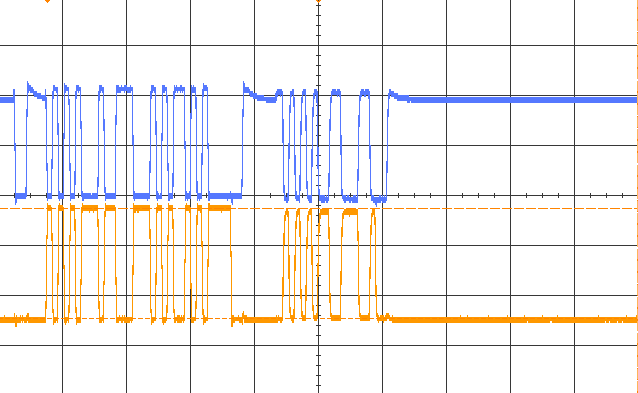
\includegraphics[width=.94\linewidth]{1}
		\caption{Packet from full speed hub}
	\end{minipage}%
	\begin{minipage}[t]{.5\textwidth}
		\centering
		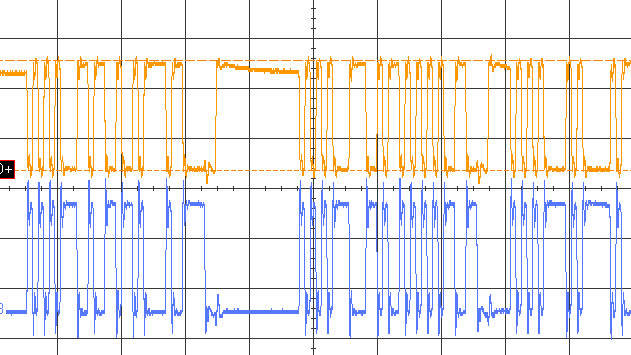
\includegraphics[width=.94\linewidth]{2}
		\caption{Packet from high speed device plugged into a full speed hub}
	\end{minipage}
\end{figure}

\begin{figure}[H]
\centering
\begin{minipage}[t]{.5\textwidth}
	\centering
	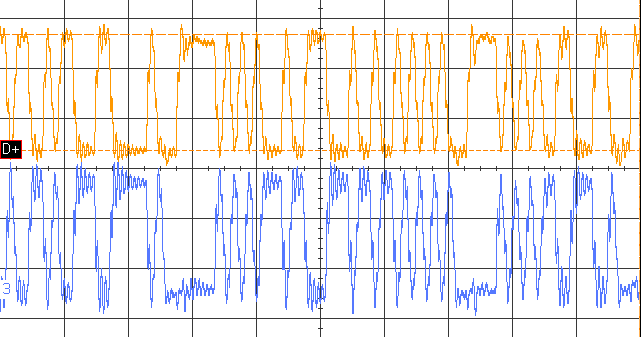
\includegraphics[width=.94\linewidth]{5}
	\caption{Packet from full speed function}
\end{minipage}%
\begin{minipage}[t]{.5\textwidth}
	\centering
	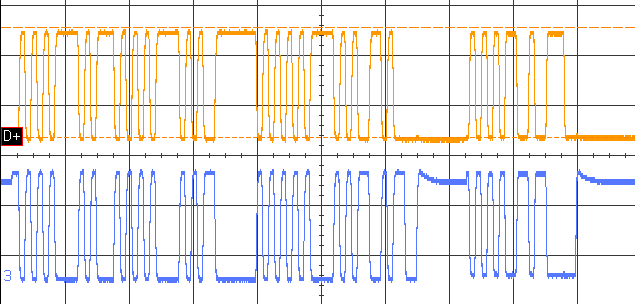
\includegraphics[width=.94\linewidth]{4}
	\caption{Packet from a low speed function}
\end{minipage}
\end{figure}

Figure 1: 0000 0001 0101 1010 SE0 - Handshake NAK

Figure 2: 0000 0001 1010 0101 0010 0011 1001 0111 SE0 - SOF

Figure 3: 0000 0001 0101 1010 SE0 - Handshake NAK

Figure 4: 0000 0001 0100 1011 SE0 - Handshake ACK\\

\sect{Analysis \& Discussion:} The waveforms matched our expectations, as the messages started with the requisite sync pattern, then went into the PID/data sections. We were able to clearly identify the start of frame and end of frame (single ended zero) easily in each of the waveforms captured.\\

\sect{Lab Questions:}

\begin{enumerate}[noitemsep,nolistsep]
	\item[\Q] Describe in detail NRZI.
	\item[\A] Non-Return to Zero Inverted code is the method of transmitting binary code used in USB signals. The signal is interpreted as a 0 when the state changes, and as a 1 when it remains constant.
	\item[\Q] How can you tell if a function is a full speed or low speed, with out looking at the waveform timing?
	\item[\A] You can look at the state of D+ and D- during idle states. This is assuming that the waveforms are labeled. If we are also missing this info, it is not possible to identify the speed of the device.
	\item[\Q] Describe what is meant by differential signaling.
	\item[\A] Differential signaling is transferring data over a line using 2 data lines. Each of the lines is the inverse of the other when transmitting data. For example, in USB, D+ being high and D- being low means that a differential 1 is being sent across the line. 
	\item[\Q] Describe bit stuffing and why it is used by USB devices.
	\item[\A] When a piece of data is being transmitted and it contains more than 6 ones in a row, the device must insert a 0 in order to keep the clock synchronized.
	\item[\Q] What is the maximum throughput in data characters per second for a full speed device, discuss the design constraints that impact this.
	\item[\A] For 8 bit characters, the throughput is approximately $1.4\times 10^{6}$ characters per second. One design constraint is the amount of overhead per message / the maximum bytes per message. Minimizing overhead is important to maximizing speed of a channel. Full speed USB has fairly low overhead when the packet is using the maximum number of bytes, so this is what we assume for our calculations. Another important constraint is the frequency with which we send data. Increases in the frequency improve the speed directly.
\end{enumerate}~

\sect{Results:} Our experiment was successful as the waveforms were successfully captured and the message types and connection speed were successfully identified.\\

\sect{Conclusions:} In this lab, we learned to capture waveforms being transmitted over a USB line and were able to identify important characteristics of that data. This will be important in future projects as the intuition behind manually translating a USB signal can be applied to hardware and software design that involves these signals. Even though manually identifying USB signals is uncommon, it is important to understand how it is being done inside different components in order to debug problems or create new technologies. 

\end{document}
